\documentclass[10pt]{article}
\usepackage{graphicx}
\usepackage{algorithm}
\usepackage{algpseudocode}

\begin{document}
\title{CSE616 Neural Networks and Their Applications\\
Assignment 3 Submission}
\author{Ayman Wagih Mohsen (2000728)}
\maketitle

\section{Question 1}
a. Predicted output with identity activation:
\[	x_1=10, y_1=5\]
\[	x_2=10, y_2=5\]
\[	h_0=1\]
\[	W_h=1, W_x=0.1, W_y=2\]
\[	h_1=W_h h_0+W_x x_1=1*1+0.1*10=2\]
\[	\hat{y}_1=W_y h_1=2*2=4\]
\[	h_2=W_h h_1+W_x x_2=1*2+0.1*10=3\]
\[	\hat{y}_2=W_y h_2=2*3=6\]

b. The total loss:
\[	L_t=\sum_i (\hat{y}_i-y_i)^2
	=(\hat{y}_1-y_1)^2+(\hat{y}_2-y_2)^2
	=(5-4)^2+(5-6)^2
	=2\]

c. Derivative of loss w.r.t. $h_1$:
\[	\frac{\partial{L_t}}{\partial{h_1}}
	=2(\hat{y}_1-y_1)W_y+2(\hat{y}_2-y_2)W_y\frac{\partial{h_2}}{\partial{h_1}}\]
\[	=2(\hat{y}_1-y_1)W_y
	+2(\hat{y}_2-y_2)W_y W_h\]
\[	=2(4-5)*2+2(6-5)*2*1=0\]

d. Derivative of loss w.r.t. $W_h$:
\[	\frac{\partial{L_t}}{\partial{W_h}}
	=2(\hat{y}_1-y_1)\frac{\partial\hat y_1}{\partial W_h}
	+2(\hat{y}_2-y_2)\frac{\partial\hat y_2}{\partial W_h}\]
\[	=2(4-5)*2+2(6-5)*6=8\]

The derivation of $\partial\hat y_1/\partial W_h$ (blue is value, green is gradient):
\begin{center}
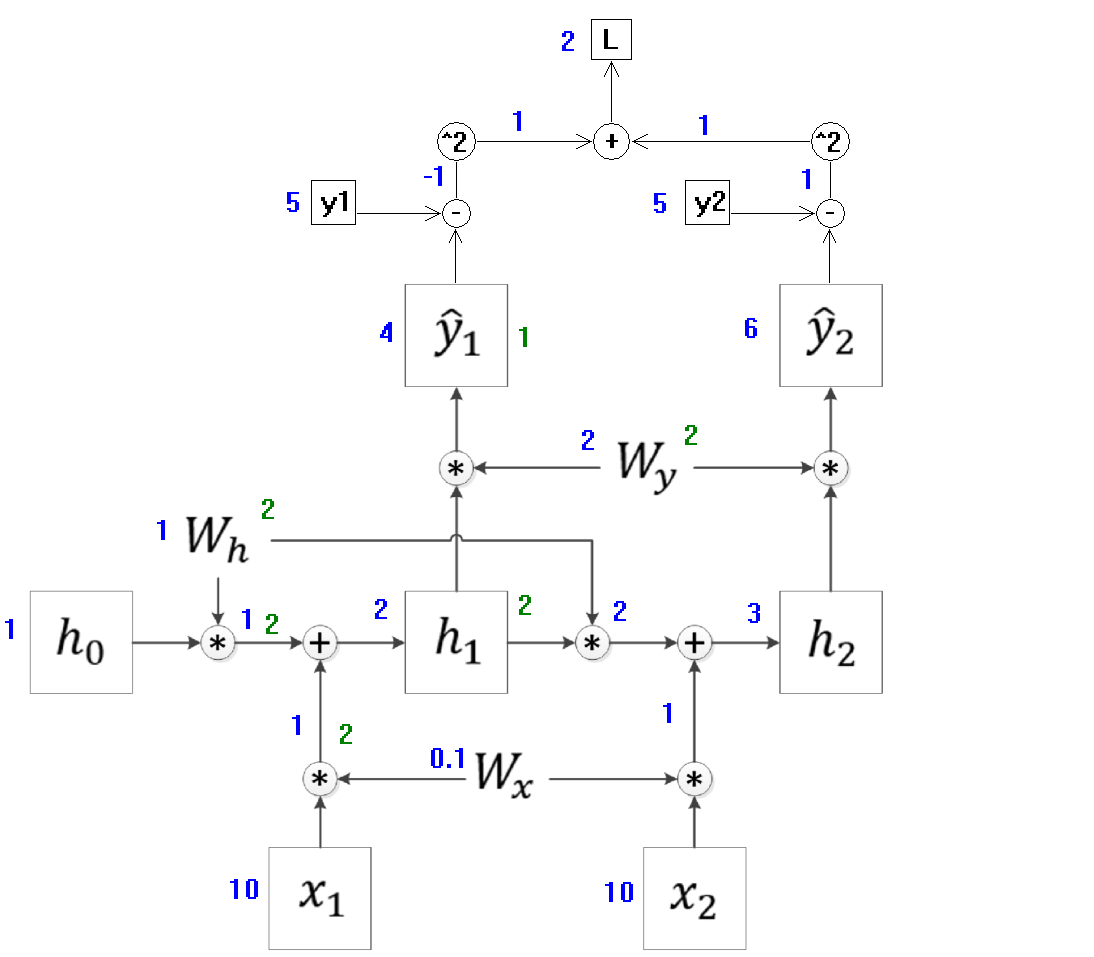
\includegraphics[width=0.9\textwidth]{20220524 Q1 attempt3a.PNG}
\DeclareGraphicsExtensions{.png}
\end{center}

The derivation of $\partial\hat y_2/\partial W_h$ (blue is value, green is gradient):
\begin{center}
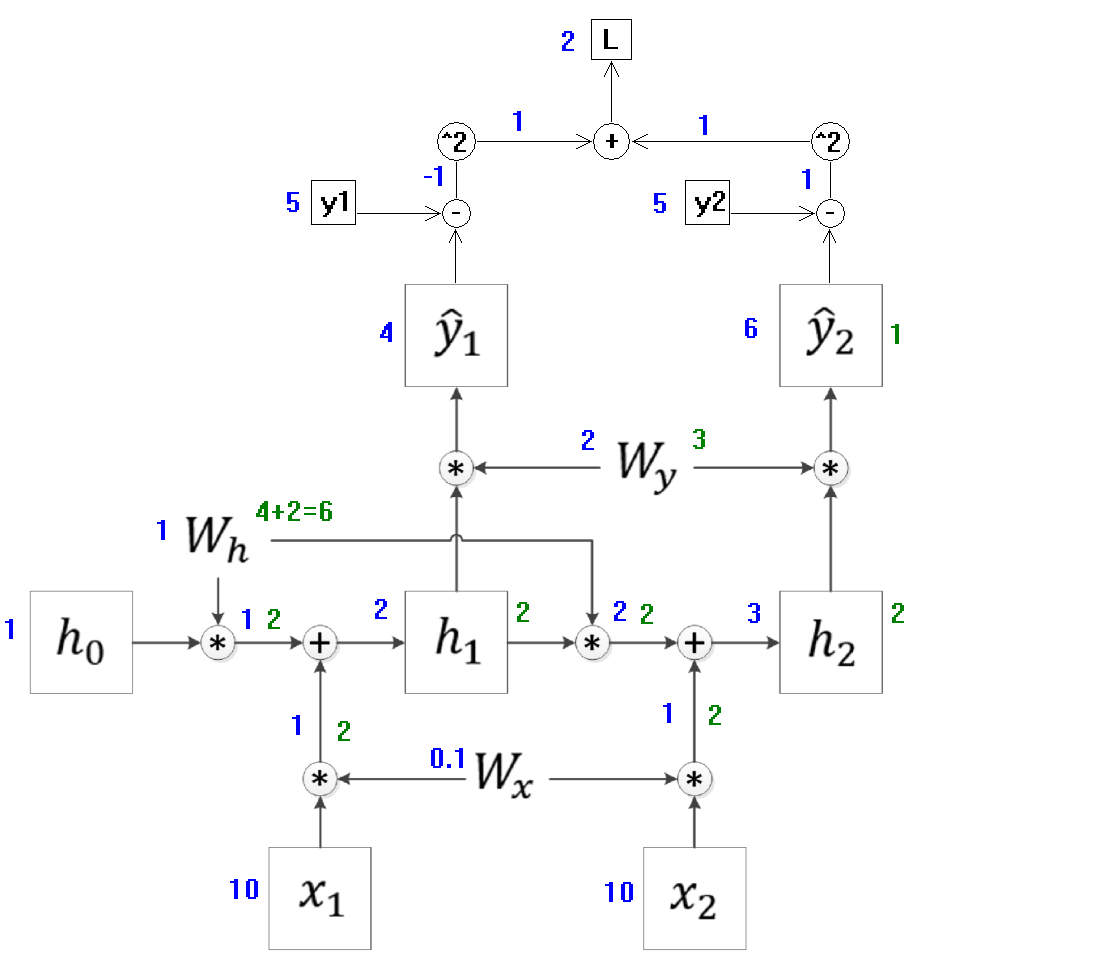
\includegraphics[width=0.9\textwidth]{20220524 Q1 attempt3b.PNG}
\DeclareGraphicsExtensions{.png}
\end{center}


\section{Question 2}
With long term dependencies that appear with a long sequence, the gradient passes by many layers, and either explodes or vanishes.
\[	h_t=tanh(W_{hh}h_{t-1}+W_{xh}x_t)\]
\begin{center}
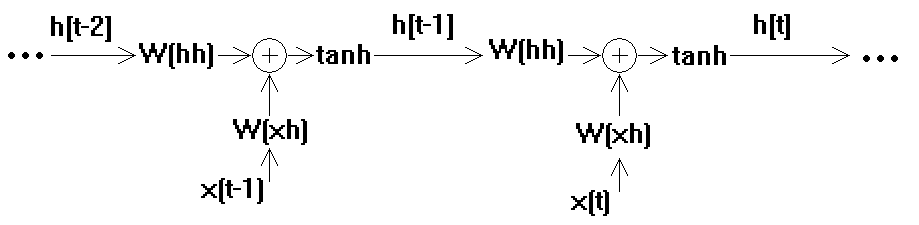
\includegraphics[width=0.9\textwidth]{20220525 1 Q2.PNG}
\DeclareGraphicsExtensions{.png}
\end{center}
The gradient becomes:
\[
	\frac{\partial J_t}{\partial W_{hh}}
	=
	\frac{\partial J_t}{\partial y_t}
	\frac{\partial y_t}{\partial h_t}
	\left(
		\sum_{k=0}^t
		\frac{\partial h_t}{\partial h_k}
		\frac{\partial h_k}{\partial W_{hh}}
	\right)
\]
\[
	=
	\frac{\partial J_t}{\partial y_t}
	\frac{\partial y_t}{\partial h_t}
	\left(
		\left(\frac{\partial h_t}{\partial h_{t-1}}...\frac{\partial h_0}{\partial W_{hh}}\right)
		+
		\left(\frac{\partial h_t}{\partial h_{t-1}}...\frac{\partial h_1}{\partial W_{hh}}\right)
		+...
		\frac{\partial h_t}{\partial W_{hh}}
	\right)
\]
And a single factor $\partial h_t/\partial h_{t-1}$ is:
\[
	\frac{\partial h_t}{\partial h_{t-1}}
	=(1-h_t^2)(W_{hh})<1
\]
So multiplying many such factors causes the gradient to vanish.

\section{Question 3}
Gated Recurrent Units (GRUs) are better than vanilla RNNs with long sequences.

\section{Question 4}
The advantage of TBTT is fast gradient calculation. The distavantage is memory loss over long time intervals.

\section{Question 5}
a. That is because an RNN may learn the statistics of the English language and have more accurate decryption. Also an RNN is better suited for handling variable-length sequences.\\
However using an FC network we can think of Caesar cipher as a 1:1 mapping of independent characters. This way, no hidden state is necessary. And the model will be simpler.\\
\\
b. The input and output are encoded as 26-dimensional vectors. Where each component represents the probability of the corresponding character.\\
\\
c. The model should have a many-to-many architecture where each output character corresponds to that character in the input.\\
\\
d. The training data should be many pairs of ciphertext and plaintext, without spaces. Such as: (khoorzruog, helloworld).\\
\\
e. The Recurrent Neural Networks are designed to handle variable length sequences. Where each output character is the result of the previous state and current input character.\\
\\
f. The tokenized characters (as numbers from 0 to 25) are then converted into vectors of 26 dimensions.\\
\\
g. The model could be as shown in Algorithm 1 below.\\
\\
h. The deciphered text characters are obtained using argmax of each vector.

\begin{algorithm}
\caption{RNN model with Keras}\label{euclid}
\begin{algorithmic}[1]
\Procedure{model\_initialization}{}
\State import tensorflow as tf
\State from tensorflow import keras
\State from tensorflow.keras import layers
\State $model = keras.Sequential()$
\State $model.add(layers.Embedding(input\_dim=26, output\_dim=26))$
\State $model.add(layers.SimpleRNN(128))$
\EndProcedure
\end{algorithmic}
\end{algorithm}

\begin{algorithm}
\caption{RNN model with Pytorch}\label{euclid}
\begin{algorithmic}[1]
\Procedure{model\_initialization}{}
\State import torch
\State from torch import nn
\State model=nn.RNN(sequence\_length, hidden\_dim, n\_layers)
\EndProcedure
\end{algorithmic}
\end{algorithm}

\end{document}



